% Options for packages loaded elsewhere
\PassOptionsToPackage{unicode}{hyperref}
\PassOptionsToPackage{hyphens}{url}
\PassOptionsToPackage{dvipsnames,svgnames,x11names}{xcolor}
%
\documentclass[
  letterpaper,
  DIV=11,
  numbers=noendperiod]{scrartcl}

\usepackage{amsmath,amssymb}
\usepackage{iftex}
\ifPDFTeX
  \usepackage[T1]{fontenc}
  \usepackage[utf8]{inputenc}
  \usepackage{textcomp} % provide euro and other symbols
\else % if luatex or xetex
  \usepackage{unicode-math}
  \defaultfontfeatures{Scale=MatchLowercase}
  \defaultfontfeatures[\rmfamily]{Ligatures=TeX,Scale=1}
\fi
\usepackage{lmodern}
\ifPDFTeX\else  
    % xetex/luatex font selection
\fi
% Use upquote if available, for straight quotes in verbatim environments
\IfFileExists{upquote.sty}{\usepackage{upquote}}{}
\IfFileExists{microtype.sty}{% use microtype if available
  \usepackage[]{microtype}
  \UseMicrotypeSet[protrusion]{basicmath} % disable protrusion for tt fonts
}{}
\makeatletter
\@ifundefined{KOMAClassName}{% if non-KOMA class
  \IfFileExists{parskip.sty}{%
    \usepackage{parskip}
  }{% else
    \setlength{\parindent}{0pt}
    \setlength{\parskip}{6pt plus 2pt minus 1pt}}
}{% if KOMA class
  \KOMAoptions{parskip=half}}
\makeatother
\usepackage{xcolor}
\setlength{\emergencystretch}{3em} % prevent overfull lines
\setcounter{secnumdepth}{-\maxdimen} % remove section numbering
% Make \paragraph and \subparagraph free-standing
\ifx\paragraph\undefined\else
  \let\oldparagraph\paragraph
  \renewcommand{\paragraph}[1]{\oldparagraph{#1}\mbox{}}
\fi
\ifx\subparagraph\undefined\else
  \let\oldsubparagraph\subparagraph
  \renewcommand{\subparagraph}[1]{\oldsubparagraph{#1}\mbox{}}
\fi

\usepackage{color}
\usepackage{fancyvrb}
\newcommand{\VerbBar}{|}
\newcommand{\VERB}{\Verb[commandchars=\\\{\}]}
\DefineVerbatimEnvironment{Highlighting}{Verbatim}{commandchars=\\\{\}}
% Add ',fontsize=\small' for more characters per line
\usepackage{framed}
\definecolor{shadecolor}{RGB}{241,243,245}
\newenvironment{Shaded}{\begin{snugshade}}{\end{snugshade}}
\newcommand{\AlertTok}[1]{\textcolor[rgb]{0.68,0.00,0.00}{#1}}
\newcommand{\AnnotationTok}[1]{\textcolor[rgb]{0.37,0.37,0.37}{#1}}
\newcommand{\AttributeTok}[1]{\textcolor[rgb]{0.40,0.45,0.13}{#1}}
\newcommand{\BaseNTok}[1]{\textcolor[rgb]{0.68,0.00,0.00}{#1}}
\newcommand{\BuiltInTok}[1]{\textcolor[rgb]{0.00,0.23,0.31}{#1}}
\newcommand{\CharTok}[1]{\textcolor[rgb]{0.13,0.47,0.30}{#1}}
\newcommand{\CommentTok}[1]{\textcolor[rgb]{0.37,0.37,0.37}{#1}}
\newcommand{\CommentVarTok}[1]{\textcolor[rgb]{0.37,0.37,0.37}{\textit{#1}}}
\newcommand{\ConstantTok}[1]{\textcolor[rgb]{0.56,0.35,0.01}{#1}}
\newcommand{\ControlFlowTok}[1]{\textcolor[rgb]{0.00,0.23,0.31}{#1}}
\newcommand{\DataTypeTok}[1]{\textcolor[rgb]{0.68,0.00,0.00}{#1}}
\newcommand{\DecValTok}[1]{\textcolor[rgb]{0.68,0.00,0.00}{#1}}
\newcommand{\DocumentationTok}[1]{\textcolor[rgb]{0.37,0.37,0.37}{\textit{#1}}}
\newcommand{\ErrorTok}[1]{\textcolor[rgb]{0.68,0.00,0.00}{#1}}
\newcommand{\ExtensionTok}[1]{\textcolor[rgb]{0.00,0.23,0.31}{#1}}
\newcommand{\FloatTok}[1]{\textcolor[rgb]{0.68,0.00,0.00}{#1}}
\newcommand{\FunctionTok}[1]{\textcolor[rgb]{0.28,0.35,0.67}{#1}}
\newcommand{\ImportTok}[1]{\textcolor[rgb]{0.00,0.46,0.62}{#1}}
\newcommand{\InformationTok}[1]{\textcolor[rgb]{0.37,0.37,0.37}{#1}}
\newcommand{\KeywordTok}[1]{\textcolor[rgb]{0.00,0.23,0.31}{#1}}
\newcommand{\NormalTok}[1]{\textcolor[rgb]{0.00,0.23,0.31}{#1}}
\newcommand{\OperatorTok}[1]{\textcolor[rgb]{0.37,0.37,0.37}{#1}}
\newcommand{\OtherTok}[1]{\textcolor[rgb]{0.00,0.23,0.31}{#1}}
\newcommand{\PreprocessorTok}[1]{\textcolor[rgb]{0.68,0.00,0.00}{#1}}
\newcommand{\RegionMarkerTok}[1]{\textcolor[rgb]{0.00,0.23,0.31}{#1}}
\newcommand{\SpecialCharTok}[1]{\textcolor[rgb]{0.37,0.37,0.37}{#1}}
\newcommand{\SpecialStringTok}[1]{\textcolor[rgb]{0.13,0.47,0.30}{#1}}
\newcommand{\StringTok}[1]{\textcolor[rgb]{0.13,0.47,0.30}{#1}}
\newcommand{\VariableTok}[1]{\textcolor[rgb]{0.07,0.07,0.07}{#1}}
\newcommand{\VerbatimStringTok}[1]{\textcolor[rgb]{0.13,0.47,0.30}{#1}}
\newcommand{\WarningTok}[1]{\textcolor[rgb]{0.37,0.37,0.37}{\textit{#1}}}

\providecommand{\tightlist}{%
  \setlength{\itemsep}{0pt}\setlength{\parskip}{0pt}}\usepackage{longtable,booktabs,array}
\usepackage{calc} % for calculating minipage widths
% Correct order of tables after \paragraph or \subparagraph
\usepackage{etoolbox}
\makeatletter
\patchcmd\longtable{\par}{\if@noskipsec\mbox{}\fi\par}{}{}
\makeatother
% Allow footnotes in longtable head/foot
\IfFileExists{footnotehyper.sty}{\usepackage{footnotehyper}}{\usepackage{footnote}}
\makesavenoteenv{longtable}
\usepackage{graphicx}
\makeatletter
\def\maxwidth{\ifdim\Gin@nat@width>\linewidth\linewidth\else\Gin@nat@width\fi}
\def\maxheight{\ifdim\Gin@nat@height>\textheight\textheight\else\Gin@nat@height\fi}
\makeatother
% Scale images if necessary, so that they will not overflow the page
% margins by default, and it is still possible to overwrite the defaults
% using explicit options in \includegraphics[width, height, ...]{}
\setkeys{Gin}{width=\maxwidth,height=\maxheight,keepaspectratio}
% Set default figure placement to htbp
\makeatletter
\def\fps@figure{htbp}
\makeatother

\KOMAoption{captions}{tableheading}
\makeatletter
\@ifpackageloaded{tcolorbox}{}{\usepackage[skins,breakable]{tcolorbox}}
\@ifpackageloaded{fontawesome5}{}{\usepackage{fontawesome5}}
\definecolor{quarto-callout-color}{HTML}{909090}
\definecolor{quarto-callout-note-color}{HTML}{0758E5}
\definecolor{quarto-callout-important-color}{HTML}{CC1914}
\definecolor{quarto-callout-warning-color}{HTML}{EB9113}
\definecolor{quarto-callout-tip-color}{HTML}{00A047}
\definecolor{quarto-callout-caution-color}{HTML}{FC5300}
\definecolor{quarto-callout-color-frame}{HTML}{acacac}
\definecolor{quarto-callout-note-color-frame}{HTML}{4582ec}
\definecolor{quarto-callout-important-color-frame}{HTML}{d9534f}
\definecolor{quarto-callout-warning-color-frame}{HTML}{f0ad4e}
\definecolor{quarto-callout-tip-color-frame}{HTML}{02b875}
\definecolor{quarto-callout-caution-color-frame}{HTML}{fd7e14}
\makeatother
\makeatletter
\makeatother
\makeatletter
\makeatother
\makeatletter
\@ifpackageloaded{caption}{}{\usepackage{caption}}
\AtBeginDocument{%
\ifdefined\contentsname
  \renewcommand*\contentsname{Table of contents}
\else
  \newcommand\contentsname{Table of contents}
\fi
\ifdefined\listfigurename
  \renewcommand*\listfigurename{List of Figures}
\else
  \newcommand\listfigurename{List of Figures}
\fi
\ifdefined\listtablename
  \renewcommand*\listtablename{List of Tables}
\else
  \newcommand\listtablename{List of Tables}
\fi
\ifdefined\figurename
  \renewcommand*\figurename{Figure}
\else
  \newcommand\figurename{Figure}
\fi
\ifdefined\tablename
  \renewcommand*\tablename{Table}
\else
  \newcommand\tablename{Table}
\fi
}
\@ifpackageloaded{float}{}{\usepackage{float}}
\floatstyle{ruled}
\@ifundefined{c@chapter}{\newfloat{codelisting}{h}{lop}}{\newfloat{codelisting}{h}{lop}[chapter]}
\floatname{codelisting}{Listing}
\newcommand*\listoflistings{\listof{codelisting}{List of Listings}}
\makeatother
\makeatletter
\@ifpackageloaded{caption}{}{\usepackage{caption}}
\@ifpackageloaded{subcaption}{}{\usepackage{subcaption}}
\makeatother
\makeatletter
\@ifpackageloaded{tcolorbox}{}{\usepackage[skins,breakable]{tcolorbox}}
\makeatother
\makeatletter
\@ifundefined{shadecolor}{\definecolor{shadecolor}{rgb}{.97, .97, .97}}
\makeatother
\makeatletter
\makeatother
\makeatletter
\makeatother
\makeatletter
\@ifpackageloaded{tikz}{}{\usepackage{tikz}}
\makeatother
        \newcommand*\circled[1]{\tikz[baseline=(char.base)]{
          \node[shape=circle,draw,inner sep=1pt] (char) {{\scriptsize#1}};}}  
                  
\ifLuaTeX
  \usepackage{selnolig}  % disable illegal ligatures
\fi
\IfFileExists{bookmark.sty}{\usepackage{bookmark}}{\usepackage{hyperref}}
\IfFileExists{xurl.sty}{\usepackage{xurl}}{} % add URL line breaks if available
\urlstyle{same} % disable monospaced font for URLs
\hypersetup{
  pdftitle={barplots and scatterplots},
  pdfauthor={Emily Malcolm-White},
  colorlinks=true,
  linkcolor={blue},
  filecolor={Maroon},
  citecolor={Blue},
  urlcolor={Blue},
  pdfcreator={LaTeX via pandoc}}

\title{barplots and scatterplots}
\author{Emily Malcolm-White}
\date{}

\begin{document}
\maketitle
\ifdefined\Shaded\renewenvironment{Shaded}{\begin{tcolorbox}[borderline west={3pt}{0pt}{shadecolor}, frame hidden, boxrule=0pt, interior hidden, enhanced, sharp corners, breakable]}{\end{tcolorbox}}\fi

\texttt{ggplot2} is a package built within the \texttt{tidyverse}
package for creating awesome graphs!

\begin{figure}

{\centering 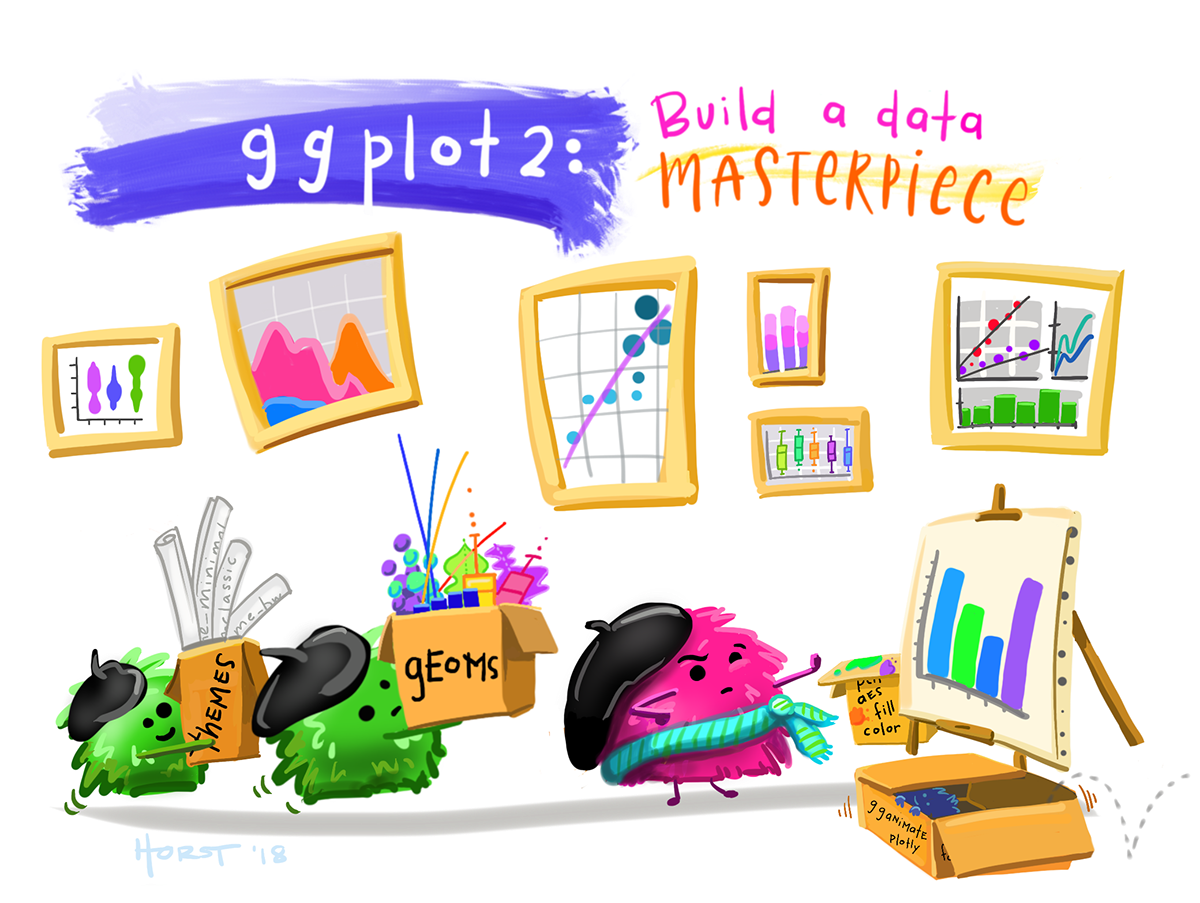
\includegraphics[width=0.5\textwidth,height=\textheight]{118_D_ggplot_files/mediabag/9a306c0a-dac8-413d-b.png}

}

\caption{Artwork by @allisonhorst}

\end{figure}

\begin{Shaded}
\begin{Highlighting}[]
\FunctionTok{library}\NormalTok{(tidyverse)}
\end{Highlighting}
\end{Shaded}

\begin{Shaded}
\begin{Highlighting}[]
\CommentTok{\#Import the can\_lang dataset }
\NormalTok{can\_lang }\OtherTok{\textless{}{-}} \FunctionTok{read.csv}\NormalTok{(}\StringTok{"https://raw.githubusercontent.com/ttimbers/canlang/master/inst/extdata/can\_lang.csv"}\NormalTok{)}
\end{Highlighting}
\end{Shaded}

\hypertarget{recall-our-top-10-example}{%
\section{Recall our Top 10 example:}\label{recall-our-top-10-example}}

This code gave a list of 10 Aboriginal Languages which have the most
number of people who speak them as their mother tongue:

\hypertarget{annotated-cell-3}{%
\label{annotated-cell-3}}%
\begin{Shaded}
\begin{Highlighting}[]
\NormalTok{ten\_lang }\OtherTok{\textless{}{-}}\NormalTok{ can\_lang }\SpecialCharTok{\%\textgreater{}\%}  \CommentTok{\#\textless{}1\textgreater{}}
  \FunctionTok{filter}\NormalTok{(category }\SpecialCharTok{==} \StringTok{"Aboriginal languages"}\NormalTok{) }\SpecialCharTok{\%\textgreater{}\%} \CommentTok{\#\textless{}2\textgreater{}}
  \FunctionTok{arrange}\NormalTok{(}\FunctionTok{desc}\NormalTok{(mother\_tongue)) }\SpecialCharTok{\%\textgreater{}\%} \CommentTok{\#\textless{}3\textgreater{}}
  \FunctionTok{select}\NormalTok{(language, mother\_tongue) }\SpecialCharTok{\%\textgreater{}\%}  \CommentTok{\#\textless{}4\textgreater{}}
  \FunctionTok{slice}\NormalTok{(}\DecValTok{1}\SpecialCharTok{:}\DecValTok{10}\NormalTok{) }\CommentTok{\#\textless{}5\textgreater{}}
\end{Highlighting}
\end{Shaded}

\begin{description}
\tightlist
\item[\circled{1}]
Start with the \texttt{can\_lang} dataset
\item[\circled{2}]
Filter for aboriginal languages only
\item[\circled{3}]
arrange the rows from highest number of people who speak the language as
their mother tongue, to the lowest number of people who speak the
language as their mother tongue
\item[\circled{4}]
only include the language and mother\_tongue columns
\item[\circled{5}]
only include the top 10 rows
\end{description}

\hypertarget{barplots}{%
\section{Barplots}\label{barplots}}

Suppose we wanted to display this information in a barplot instead of in
a table. Let's take a look at the \texttt{ggplot} syntax:

\begin{figure}

{\centering 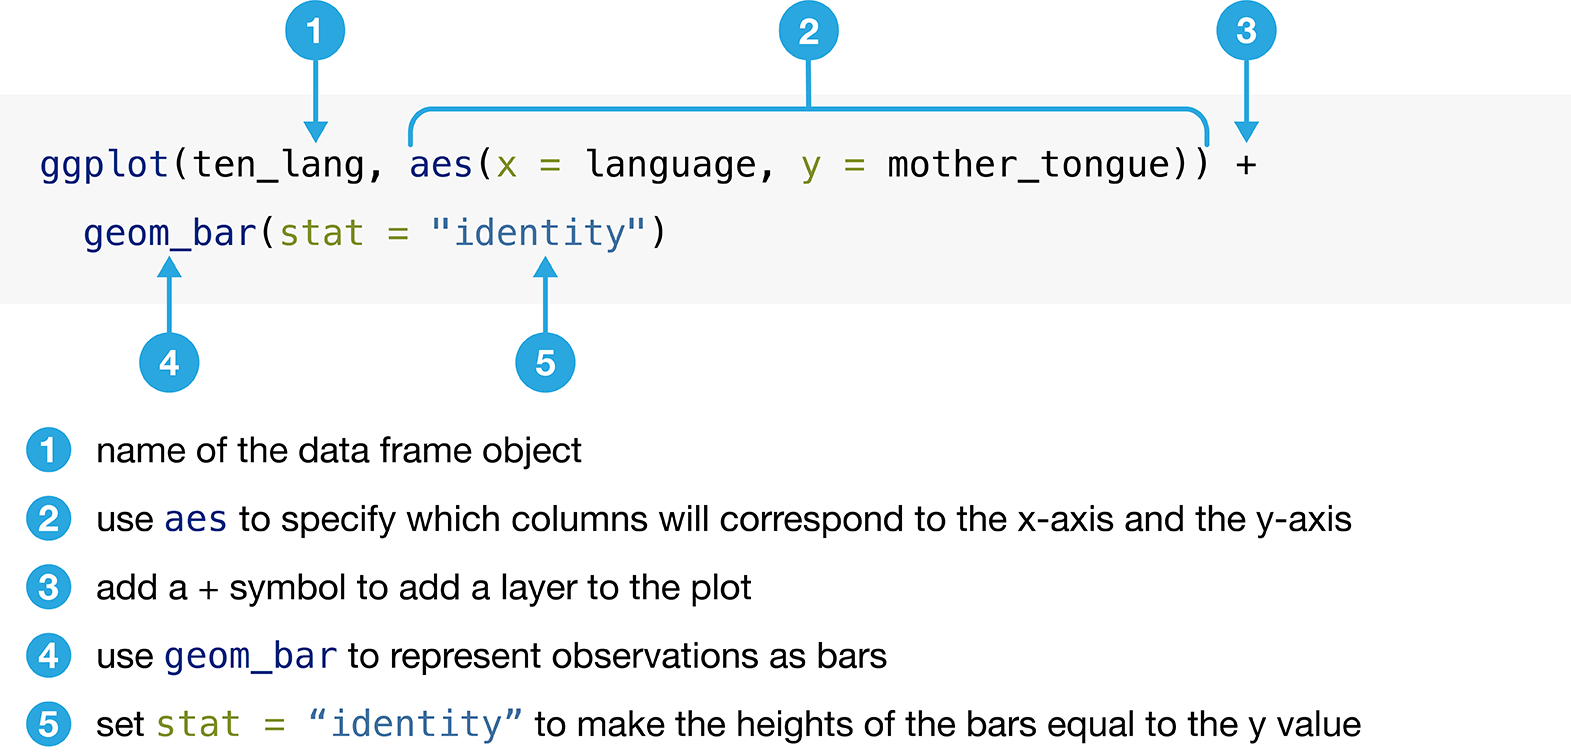
\includegraphics{118_D_ggplot_files/mediabag/ggplot_function.png}

}

\caption{Credit:
https://github.com/UBC-DSCI/introduction-to-datascience/}

\end{figure}

\hypertarget{annotated-cell-4}{%
\label{annotated-cell-4}}%
\begin{Shaded}
\begin{Highlighting}[]
\NormalTok{ten\_lang }\SpecialCharTok{\%\textgreater{}\%} \CommentTok{\#\textless{}1\textgreater{} }
  \FunctionTok{ggplot}\NormalTok{(}\FunctionTok{aes}\NormalTok{(}\AttributeTok{x =}\NormalTok{ language, }\AttributeTok{y =}\NormalTok{ mother\_tongue)) }\SpecialCharTok{+} \CommentTok{\#\textless{}2\textgreater{} }
  \FunctionTok{geom\_bar}\NormalTok{(}\AttributeTok{stat =} \StringTok{"identity"}\NormalTok{) }\CommentTok{\#\textless{}3\textgreater{}}
\end{Highlighting}
\end{Shaded}

\begin{description}
\tightlist
\item[\circled{1}]
Begin with the \texttt{ten\_lang} dataset
\item[\circled{2}]
Create a plot -- the x-axis contains the languages and the y-axis
contains the number of people who speak the language as their mother
tongue. This sets up the coordinate system, but no visualization appears
yet.
\item[\circled{3}]
add a layer with a barplot. The height of the bars should simply be the
number of people who speak the language as their mother tongue. Without
\texttt{stat\ =\ "identity"}, \texttt{geom\_bar()} defaults to
\texttt{stat\ =\ "count"}, which means it counts rows instead of using a
y-variable.
\end{description}

\begin{figure}[H]

{\centering 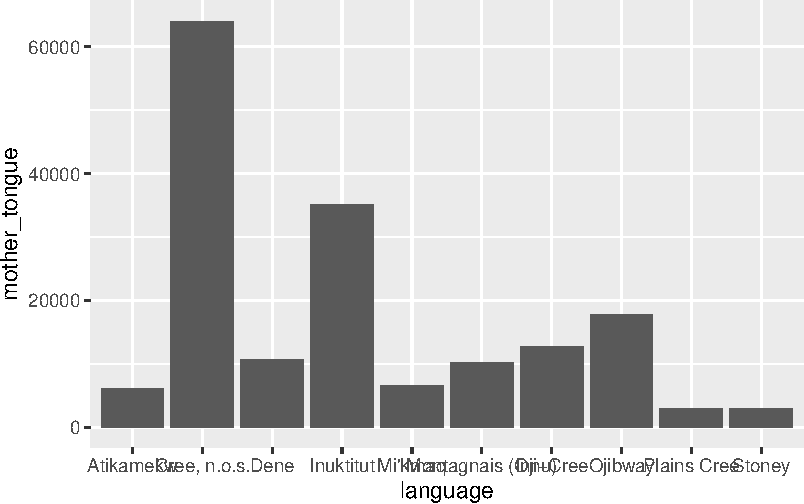
\includegraphics{118_D_ggplot_files/figure-pdf/unnamed-chunk-4-1.pdf}

}

\end{figure}

Is there any improvements we could make to this graph?

\hypertarget{to-better-view-text}{%
\section{To better view text}\label{to-better-view-text}}

Display the bars horizontally instead of vertically!

\hypertarget{annotated-cell-5}{%
\label{annotated-cell-5}}%
\begin{Shaded}
\begin{Highlighting}[]
\FunctionTok{ggplot}\NormalTok{(ten\_lang, }\FunctionTok{aes}\NormalTok{(}\AttributeTok{x =}\NormalTok{ language, }\AttributeTok{y =}\NormalTok{ mother\_tongue)) }\SpecialCharTok{+}
  \FunctionTok{geom\_bar}\NormalTok{(}\AttributeTok{stat =} \StringTok{"identity"}\NormalTok{) }\SpecialCharTok{+}  
  \FunctionTok{coord\_flip}\NormalTok{() }\CommentTok{\#\textless{}1\textgreater{}}
\end{Highlighting}
\end{Shaded}

\begin{description}
\tightlist
\item[\circled{1}]
This flips the x and y axes!
\end{description}

\begin{figure}[H]

{\centering 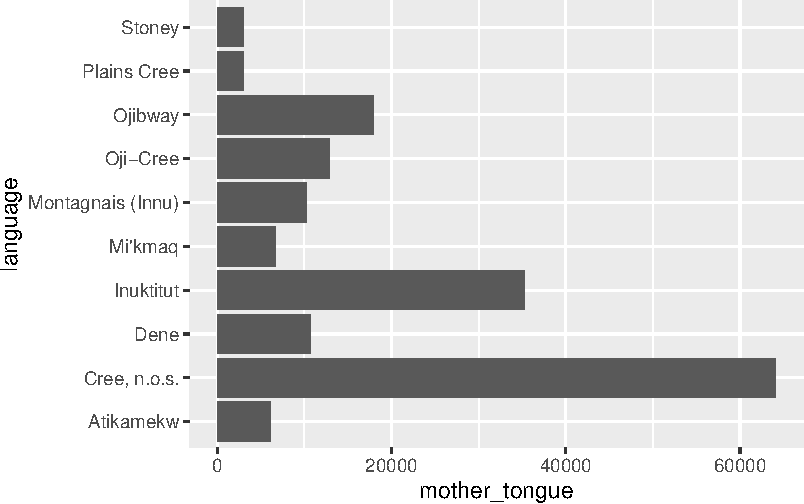
\includegraphics{118_D_ggplot_files/figure-pdf/unnamed-chunk-5-1.pdf}

}

\end{figure}

\begin{Shaded}
\begin{Highlighting}[]
\CommentTok{\#OR}

\FunctionTok{ggplot}\NormalTok{(ten\_lang, }\FunctionTok{aes}\NormalTok{(}\AttributeTok{x =}\NormalTok{ mother\_tongue, }\AttributeTok{y =}\NormalTok{ language)) }\SpecialCharTok{+}
  \FunctionTok{geom\_bar}\NormalTok{(}\AttributeTok{stat =} \StringTok{"identity"}\NormalTok{) }
\end{Highlighting}
\end{Shaded}

\begin{figure}[H]

{\centering 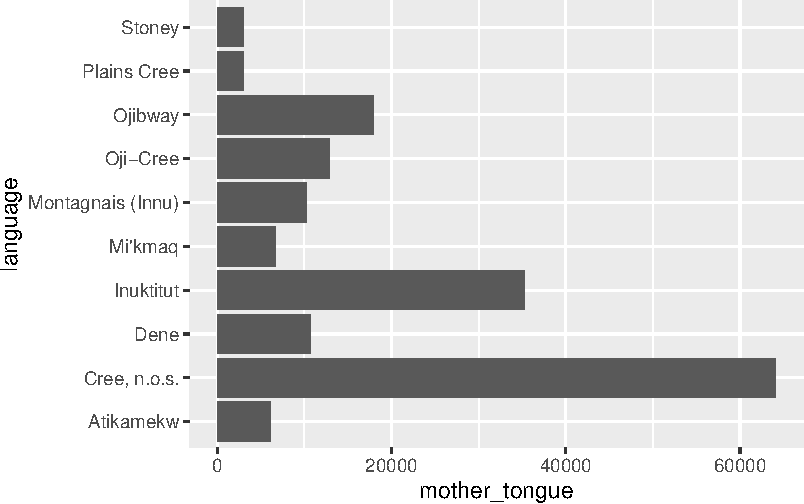
\includegraphics{118_D_ggplot_files/figure-pdf/unnamed-chunk-5-2.pdf}

}

\end{figure}

\hypertarget{labels-colors-and-themes}{%
\section{Labels, Colors, and Themes}\label{labels-colors-and-themes}}

\hypertarget{annotated-cell-7}{%
\label{annotated-cell-7}}%
\begin{Shaded}
\begin{Highlighting}[]
\FunctionTok{ggplot}\NormalTok{(ten\_lang, }\FunctionTok{aes}\NormalTok{(}\AttributeTok{x =}\NormalTok{ mother\_tongue, }\AttributeTok{y =} \FunctionTok{reorder}\NormalTok{(language, mother\_tongue))) }\SpecialCharTok{+} \CommentTok{\#\textless{}1\textgreater{}}
  \FunctionTok{geom\_bar}\NormalTok{(}\AttributeTok{fill=}\StringTok{"lightblue"}\NormalTok{, }\AttributeTok{stat =} \StringTok{"identity"}\NormalTok{) }\SpecialCharTok{+} \CommentTok{\#\textless{}2\textgreater{} }
  \FunctionTok{ylab}\NormalTok{(}\StringTok{"Language"}\NormalTok{) }\SpecialCharTok{+} \CommentTok{\#\textless{}3\textgreater{} }
  \FunctionTok{xlab}\NormalTok{(}\StringTok{"Mother Tongue (Number of Canadian Residents)"}\NormalTok{) }\SpecialCharTok{+} \CommentTok{\#\textless{}4\textgreater{}}
  \FunctionTok{ggtitle}\NormalTok{(}\StringTok{"Ten Aboriginal Languages Most Often }\SpecialCharTok{\textbackslash{}n}\StringTok{ Reported by Canadian Residents }\SpecialCharTok{\textbackslash{}n}\StringTok{ as Their Mother Tongue"}\NormalTok{) }\SpecialCharTok{+} \CommentTok{\#\textless{}5\textgreater{}}
  \FunctionTok{theme\_minimal}\NormalTok{() }\CommentTok{\#\textless{}6\textgreater{}}
\end{Highlighting}
\end{Shaded}

\begin{description}
\tightlist
\item[\circled{1}]
The reorder function helps to reorder the languages from highest to
lowest value of mother tongue.
\item[\circled{2}]
Changes the colors of the bars to light blue!
\item[\circled{3}]
Updates x-axis label
\item[\circled{4}]
Updates y-axis label
\item[\circled{5}]
adds a title
\item[\circled{6}]
changes the theme
\end{description}

\begin{figure}[H]

{\centering 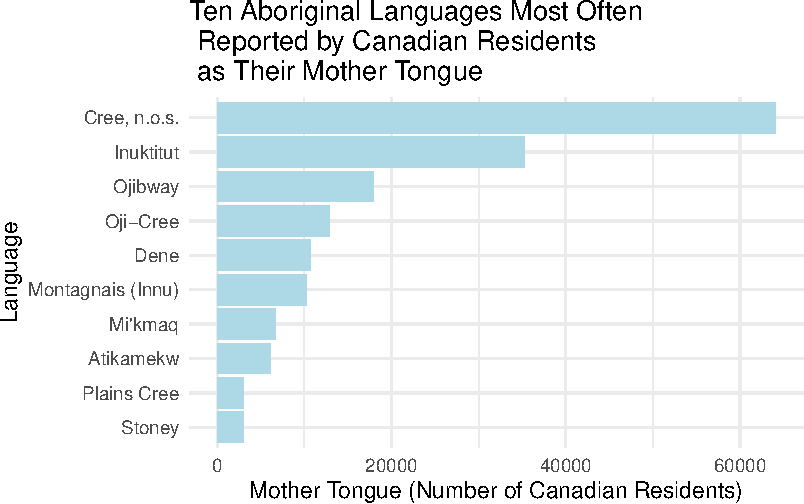
\includegraphics{118_D_ggplot_files/figure-pdf/unnamed-chunk-6-1.pdf}

}

\end{figure}

\begin{tcolorbox}[enhanced jigsaw, coltitle=black, leftrule=.75mm, toprule=.15mm, colframe=quarto-callout-tip-color-frame, breakable, bottomrule=.15mm, colbacktitle=quarto-callout-tip-color!10!white, bottomtitle=1mm, toptitle=1mm, titlerule=0mm, arc=.35mm, rightrule=.15mm, title=\textcolor{quarto-callout-tip-color}{\faLightbulb}\hspace{0.5em}{Tip}, colback=white, left=2mm, opacitybacktitle=0.6, opacityback=0]

Barplots are good for displaying one categorical variable and one
numeric variable. The number variable could be counts (as above) or they
could be averages or totals or maximums or minimums (or many other
things!)

\end{tcolorbox}

\hypertarget{ggplot-scatterplot-with-geom_point}{%
\section{\texorpdfstring{ggplot: scatterplot with
\texttt{geom\_point}}{ggplot: scatterplot with geom\_point}}\label{ggplot-scatterplot-with-geom_point}}

\begin{tcolorbox}[enhanced jigsaw, coltitle=black, leftrule=.75mm, toprule=.15mm, colframe=quarto-callout-tip-color-frame, breakable, bottomrule=.15mm, colbacktitle=quarto-callout-tip-color!10!white, bottomtitle=1mm, toptitle=1mm, titlerule=0mm, arc=.35mm, rightrule=.15mm, title=\textcolor{quarto-callout-tip-color}{\faLightbulb}\hspace{0.5em}{Tip}, colback=white, left=2mm, opacitybacktitle=0.6, opacityback=0]

Scatterplots are good for displaying the relationship between two
numerical variables.

\end{tcolorbox}

The \texttt{mtcars} dataset was extracted from the 1974 Motor Trend US
magazine, and comprises fuel consumption and 10 aspects of automobile
design and performance for 32 automobiles (1973--74 models). It's
available inside the \texttt{ggplot} package which is already installed.

\begin{Shaded}
\begin{Highlighting}[]
\CommentTok{\#load the data}
\FunctionTok{data}\NormalTok{(mtcars)}
\end{Highlighting}
\end{Shaded}

\hypertarget{annotated-cell-9}{%
\label{annotated-cell-9}}%
\begin{Shaded}
\begin{Highlighting}[]
\NormalTok{mtcars }\SpecialCharTok{\%\textgreater{}\%} \CommentTok{\#\textless{}1\textgreater{}}
\FunctionTok{ggplot}\NormalTok{(}\FunctionTok{aes}\NormalTok{(}\AttributeTok{x=}\NormalTok{wt, }\AttributeTok{y=}\NormalTok{mpg)) }\SpecialCharTok{+} \CommentTok{\#\textless{}2\textgreater{}}
  \FunctionTok{geom\_point}\NormalTok{() }\CommentTok{\#\textless{}3\textgreater{}}
\end{Highlighting}
\end{Shaded}

\begin{description}
\tightlist
\item[\circled{1}]
Begin with the \texttt{mtcars} dataset
\item[\circled{2}]
set up the plot -- weight on the x-axis and miles per gallon on the
y-axis
\item[\circled{3}]
Adds a scatter plot layer to the plot.
\end{description}

\begin{figure}[H]

{\centering 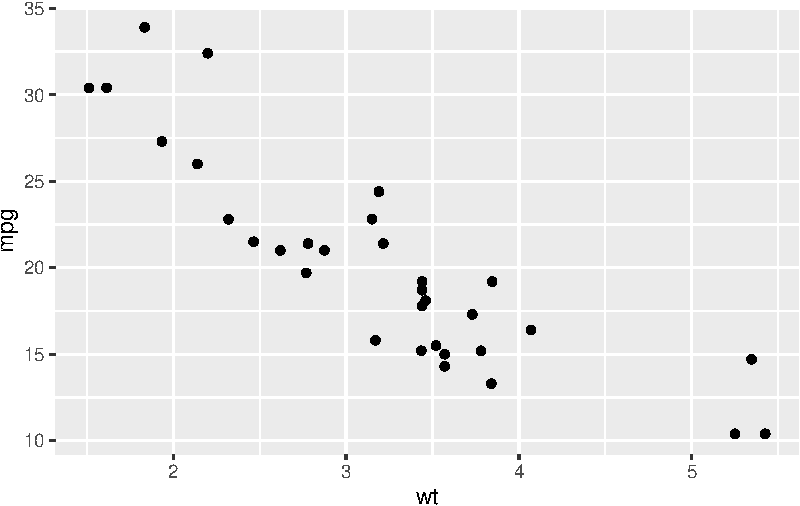
\includegraphics{118_D_ggplot_files/figure-pdf/unnamed-chunk-8-1.pdf}

}

\end{figure}

Note that you can change the color, shape (\texttt{pch} for plotting
character) and size of these points!

\hypertarget{quick-update-to-the-dataset}{%
\subsubsection{Quick update to the
dataset}\label{quick-update-to-the-dataset}}

\begin{Shaded}
\begin{Highlighting}[]
\CommentTok{\#code to update \textasciigrave{}mtcars\textasciigrave{} dataset so that \textasciigrave{}am\textasciigrave{} is treated as a factor rather than a continuous numeric variable}
\NormalTok{mtcars }\OtherTok{\textless{}{-}}\NormalTok{ mtcars }\SpecialCharTok{\%\textgreater{}\%}  
  \FunctionTok{mutate}\NormalTok{(}\AttributeTok{am =} \FunctionTok{as.factor}\NormalTok{(am)) }
\end{Highlighting}
\end{Shaded}

This modifies the am column, which represents the transmission type of
the car (0 = automatic, 1 = manual). The as.factor(am) function converts
the am variable from a numeric type (0 or 1) into a categorical factor.

\hypertarget{inside-aes-or-outside-aes}{%
\section{\texorpdfstring{Inside \texttt{aes()} or outside
\texttt{aes()}?}{Inside aes() or outside aes()?}}\label{inside-aes-or-outside-aes}}

What is the difference between these two graphs?

\hypertarget{annotated-cell-11}{%
\label{annotated-cell-11}}%
\begin{Shaded}
\begin{Highlighting}[]
\CommentTok{\#color not in aesthetics}
\FunctionTok{ggplot}\NormalTok{(mtcars, }\FunctionTok{aes}\NormalTok{(}\AttributeTok{x=}\NormalTok{wt, }\AttributeTok{y=}\NormalTok{mpg)) }\SpecialCharTok{+}
  \FunctionTok{geom\_point}\NormalTok{(}\AttributeTok{color=}\StringTok{"red"}\NormalTok{) }\CommentTok{\#\textless{}1\textgreater{}}
\end{Highlighting}
\end{Shaded}

\begin{description}
\tightlist
\item[\circled{1}]
color the same for all points
\end{description}

\begin{figure}[H]

{\centering 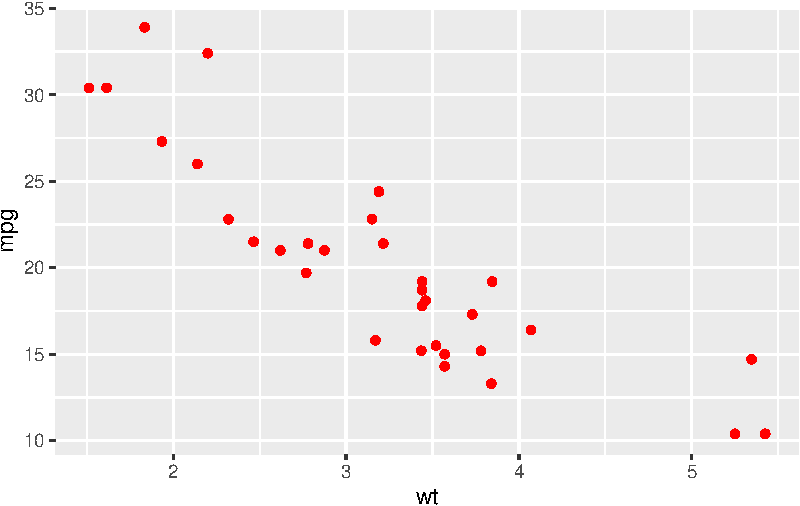
\includegraphics{118_D_ggplot_files/figure-pdf/unnamed-chunk-10-1.pdf}

}

\end{figure}

\hypertarget{annotated-cell-12}{%
\label{annotated-cell-12}}%
\begin{Shaded}
\begin{Highlighting}[]
\CommentTok{\#color in aesthetics}
\FunctionTok{ggplot}\NormalTok{(mtcars, }\FunctionTok{aes}\NormalTok{(}\AttributeTok{x=}\NormalTok{wt, }\AttributeTok{y=}\NormalTok{mpg)) }\SpecialCharTok{+}
  \FunctionTok{geom\_point}\NormalTok{(}\FunctionTok{aes}\NormalTok{(}\AttributeTok{color=}\NormalTok{am)) }\CommentTok{\#\textless{}1\textgreater{}}
\end{Highlighting}
\end{Shaded}

\begin{description}
\tightlist
\item[\circled{1}]
color will vary based on the value of am
\end{description}

\begin{figure}[H]

{\centering 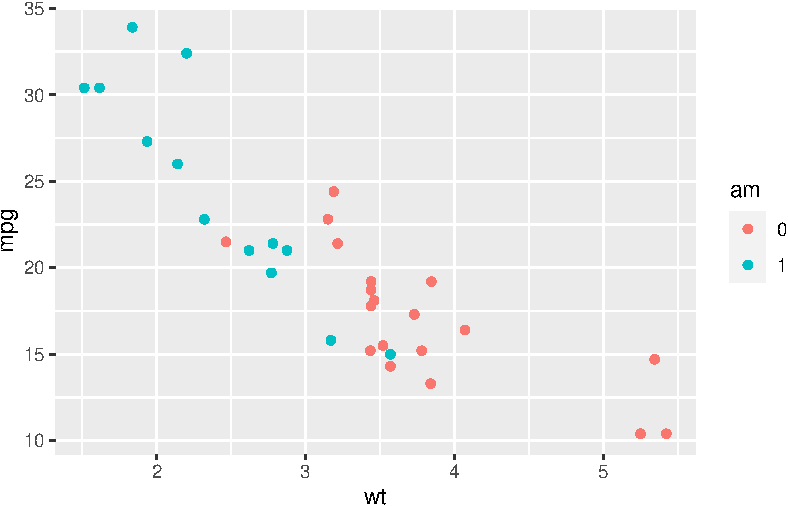
\includegraphics{118_D_ggplot_files/figure-pdf/unnamed-chunk-11-1.pdf}

}

\end{figure}

\begin{tcolorbox}[enhanced jigsaw, coltitle=black, leftrule=.75mm, toprule=.15mm, colframe=quarto-callout-tip-color-frame, breakable, bottomrule=.15mm, colbacktitle=quarto-callout-tip-color!10!white, bottomtitle=1mm, toptitle=1mm, titlerule=0mm, arc=.35mm, rightrule=.15mm, title=\textcolor{quarto-callout-tip-color}{\faLightbulb}\hspace{0.5em}{Tip}, colback=white, left=2mm, opacitybacktitle=0.6, opacityback=0]

\begin{itemize}
\tightlist
\item
  If the thing you are trying to change (color, shape, size, etc.)
  depends on a variable, you should put in \emph{inside} the aesthetics
\item
  If the thing you are trying to change (color, shape, size, etc.)
  should happen for all things, you should not put it inside the
  aesthetics.
\end{itemize}

\end{tcolorbox}

\hypertarget{customizing-colors-in-aesthetics}{%
\section{Customizing Colors in
Aesthetics}\label{customizing-colors-in-aesthetics}}

\hypertarget{annotated-cell-13}{%
\label{annotated-cell-13}}%
\begin{Shaded}
\begin{Highlighting}[]
\CommentTok{\#color in aesthetics}
\FunctionTok{ggplot}\NormalTok{(mtcars, }\FunctionTok{aes}\NormalTok{(}\AttributeTok{x=}\NormalTok{wt, }\AttributeTok{y=}\NormalTok{mpg)) }\SpecialCharTok{+}
  \FunctionTok{geom\_point}\NormalTok{(}\FunctionTok{aes}\NormalTok{(}\AttributeTok{color=}\NormalTok{am)) }\SpecialCharTok{+}
  \FunctionTok{scale\_color\_manual}\NormalTok{(}\AttributeTok{values=}\FunctionTok{c}\NormalTok{(}\StringTok{"black"}\NormalTok{, }\StringTok{"orange"}\NormalTok{)) }\CommentTok{\#\textless{}1\textgreater{}}
\end{Highlighting}
\end{Shaded}

\begin{description}
\tightlist
\item[\circled{1}]
This updates the two colors to black and orange, instead of the default
colors.
\end{description}

\begin{figure}[H]

{\centering 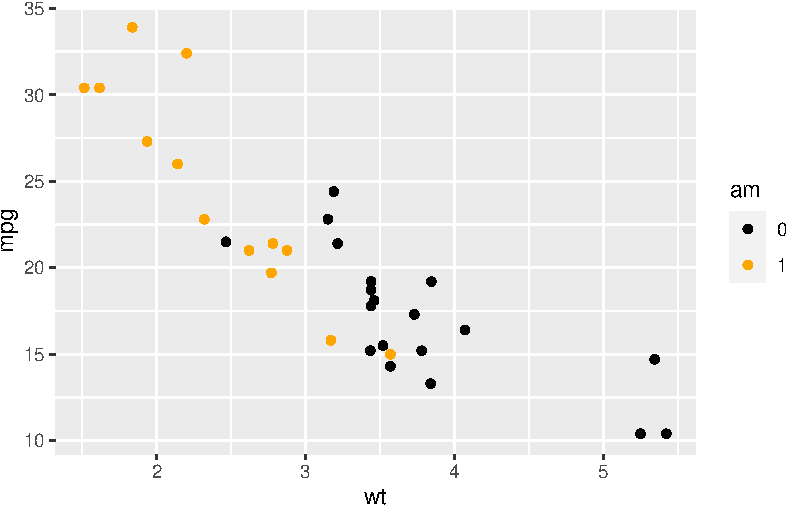
\includegraphics{118_D_ggplot_files/figure-pdf/unnamed-chunk-12-1.pdf}

}

\end{figure}

\hypertarget{global-vs.-local-aesthetics}{%
\section{Global vs.~Local
Aesthetics}\label{global-vs.-local-aesthetics}}

Global aesthetic mappings apply to all geometries and can be defined
when you initially call \texttt{ggplot()}. All the geometries added as
layers will default to this mapping. Local aesthetic mappings add
additional information or override the default mappings.

\begin{Shaded}
\begin{Highlighting}[]
\CommentTok{\#color = am as a global aethetic}
\FunctionTok{ggplot}\NormalTok{(mtcars, }\FunctionTok{aes}\NormalTok{(}\AttributeTok{x=}\NormalTok{wt, }\AttributeTok{y=}\NormalTok{mpg, }\AttributeTok{color=}\NormalTok{am)) }\SpecialCharTok{+}
  \FunctionTok{geom\_point}\NormalTok{()}
\end{Highlighting}
\end{Shaded}

\begin{figure}[H]

{\centering 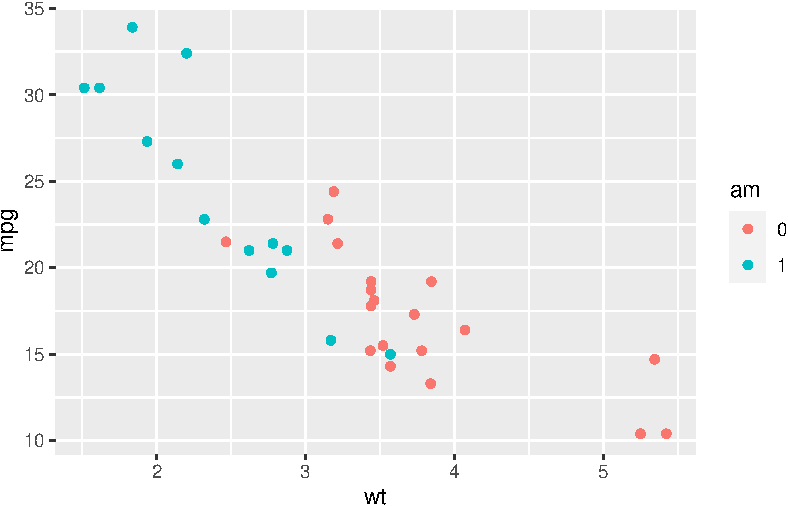
\includegraphics{118_D_ggplot_files/figure-pdf/unnamed-chunk-13-1.pdf}

}

\end{figure}

\begin{Shaded}
\begin{Highlighting}[]
\CommentTok{\#color = am as a local aethetic}
\FunctionTok{ggplot}\NormalTok{(mtcars, }\FunctionTok{aes}\NormalTok{(}\AttributeTok{x=}\NormalTok{wt, }\AttributeTok{y=}\NormalTok{mpg)) }\SpecialCharTok{+}
  \FunctionTok{geom\_point}\NormalTok{(}\FunctionTok{aes}\NormalTok{(}\AttributeTok{color=}\NormalTok{am))}
\end{Highlighting}
\end{Shaded}

\begin{figure}[H]

{\centering 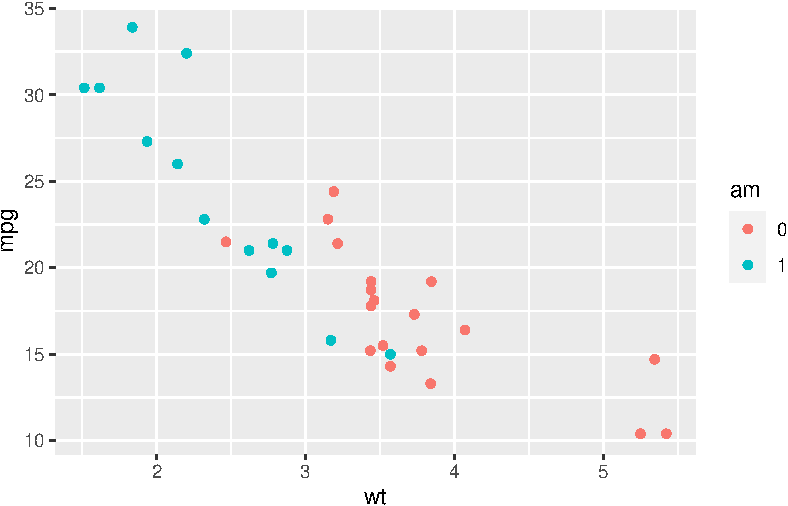
\includegraphics{118_D_ggplot_files/figure-pdf/unnamed-chunk-14-1.pdf}

}

\end{figure}

\begin{Shaded}
\begin{Highlighting}[]
\CommentTok{\#overwriting color = am as a global aethetic with a local aesthetic}
\FunctionTok{ggplot}\NormalTok{(mtcars, }\FunctionTok{aes}\NormalTok{(}\AttributeTok{x=}\NormalTok{wt, }\AttributeTok{y=}\NormalTok{mpg, }\AttributeTok{color=}\NormalTok{am)) }\SpecialCharTok{+}
  \FunctionTok{geom\_point}\NormalTok{(}\AttributeTok{color=}\StringTok{"purple"}\NormalTok{)}
\end{Highlighting}
\end{Shaded}

\begin{figure}[H]

{\centering 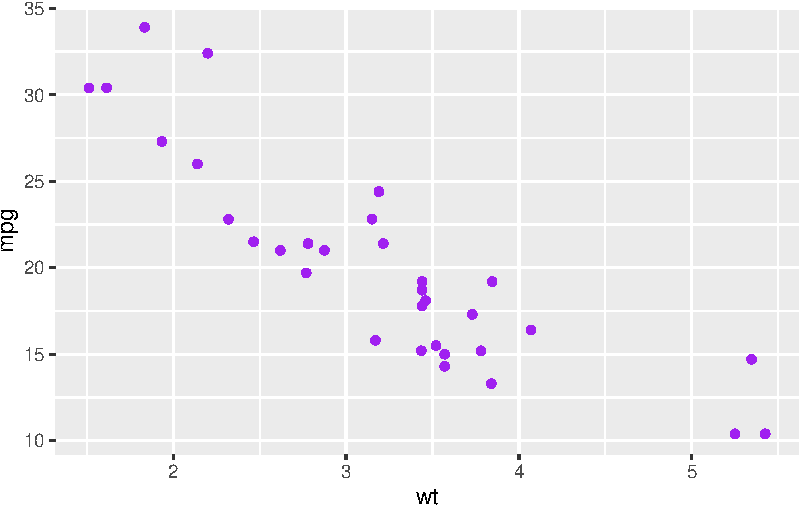
\includegraphics{118_D_ggplot_files/figure-pdf/unnamed-chunk-15-1.pdf}

}

\end{figure}



\end{document}
